\documentclass[11pt]{article}

\usepackage[margin=1in]{geometry}
\usepackage{amsmath,amssymb,bm}
\usepackage{hyperref}
\usepackage{booktabs}
\usepackage{graphicx}
\usepackage{xcolor}
\usepackage{listings}
\usepackage{natbib}
\usepackage{algorithm}
\usepackage{algpseudocode}
\usepackage{microtype}

\lstset{
    basicstyle=\ttfamily\small,
    breaklines=true,
    columns=fullflexible,
    frame=single,
    backgroundcolor=\color{gray!8},
}

\title{\textbf{pyTIDES}: A Python Framework for High-Order Taylor Integration\\
of Hierarchical Planetary and Stellar Systems}

\author{%
  % TODO: fill in author name(s), affiliation(s), ORCID(s), and corresponding email.
  Carlos Vázquez Monzón\thanks{PDI en la Universidad de Loyola, Dos Hermanas, Sevilla (Spain)} \\
  \texttt{cvazquez@uloloya.es}
}

\date{\today}

\begin{document}
\maketitle

\begin{abstract}
We present \texttt{pyTIDES}, distributed as the Python package
\texttt{exotides}, a Python-native framework for the high-order Taylor
integration of hierarchical planetary and stellar systems. The software
combines a generic variable-order, variable-step Taylor-series ordinary
differential equation solver with a direct Newtonian $N$-body model and a
hierarchy-aware layer that constructs dynamically consistent barycentric
initial conditions from trees of Keplerian orbits. The Taylor engine follows
the TIDES approach of generating normalized derivatives recursively through
elementary series operations and supports both double-precision and
arbitrary-precision arithmetic. For astrophysical applications,
\texttt{pyTIDES} provides a catalog of named star--planet--moon, binary-star,
and triple-star architectures; a Jacobi-like interior-reference convention
for converting hierarchical orbital elements into Cartesian states;
dense-output event detection; an optional pairwise first post-Newtonian
correction; and an optional Numba-accelerated Newtonian path. The numerical
engine itself is not restricted to hierarchical systems, whereas the
high-level construction and diagnostic tools are deliberately designed for
systems possessing a meaningful orbital hierarchy. This paper describes the
numerical method, formalizes the hierarchical initial-condition algorithm,
documents the physical scope of the package, and places \texttt{pyTIDES} in
the context of existing Taylor and $N$-body software. All reported
experiments are generated by versioned, rerunnable scripts distributed with
the software (\texttt{docs/paper\_experiments/}): tolerance convergence for a
Kepler orbit in both double and 200-bit arbitrary precision, energy/angular-momentum
conservation distinguishing truncation- and round-off-dominated regimes, a
from-scratch independent reconstruction of the hierarchical initial-condition
algorithm, convergence of the 1PN apsidal-precession correction, hierarchical
and non-hierarchical reference problems (Kozai--Lidov cycling; the
Pythagorean three-body problem), event-localization accuracy, and a
matched-accuracy performance comparison against REBOUND. The independent
reconstruction of the hierarchy algorithm uncovered a genuine defect in the
previously released barycentric-construction routine, affecting every
catalog configuration nested three levels or deeper; this revision documents,
fixes, and re-verifies it as part of the validation itself, to machine
precision across the full 22-template catalog.
\end{abstract}


%==============================================================================
\section{Introduction}
%==============================================================================

Accurate numerical integration is central to celestial mechanics and
exoplanet dynamics. Depending on the scientific problem, commonly used
approaches include symplectic mappings for long-term nearly Hamiltonian
evolution, high-order adaptive integrators for strongly varying timescales,
secular approximations for hierarchical systems, and direct $N$-body
integration when the full orbital phase information is required.
Taylor-series methods provide a complementary strategy: instead of
constructing a step from a fixed number of stage evaluations, they generate a
local power-series representation of the solution and use high-order
derivatives of the equations of motion to advance the state.

The TIDES framework formalized this approach for general systems of ordinary
differential equations (ODEs), using recurrence relations for normalized
derivatives to construct Taylor coefficients efficiently \citep{Abad2012}.
Modern work has demonstrated that high-order Taylor methods can be highly
competitive in astrodynamics, particularly when combined with symbolic
decomposition, just-in-time compilation, and robust dense-output event
detection \citep{Biscani2021,Biscani2022}. Nevertheless, the original TIDES
software ecosystem is centered on compiled-language libraries and
code-generation tools. To the best of our knowledge, there is no maintained
Python-native reimplementation of the original TIDES framework intended to
expose the method directly as readable Python software.

We introduce \texttt{pyTIDES}, whose installable package is named
\texttt{exotides}. The project has two principal aims. First, it provides a
from-scratch Python implementation of a variable-order, variable-step
Taylor-series ODE solver based on the TIDES methodology, with dense output,
event detection, and optional arbitrary-precision arithmetic. Second, it
provides an astrophysical construction layer for hierarchical planetary and
stellar systems. A user can specify a system as a tree of named bodies and
Keplerian elements, while the package determines the appropriate interior
reference for each orbit and assembles a global barycentric Cartesian state.

The second aim addresses a practical distinction between a numerical
integrator and a usable orbital-dynamics workflow. General-purpose $N$-body
packages usually accept Cartesian states or provide low-level orbital-element
conversion utilities, but the physical meaning of an orbit in a hierarchy can
depend on more than a body's immediate parent. For example, the outer member
of a nested stellar triple should orbit the barycenter and combined mass of
the inner subsystem. Likewise, a circumbinary planet is naturally referenced
to the binary barycenter rather than to either stellar component
individually. \texttt{pyTIDES} makes this hierarchy explicit and applies a
single interior-reference convention consistently to initialization and
diagnostics.

The package is deliberately not positioned as a replacement for mature
general-purpose tools such as REBOUND or for highly optimized Taylor software
such as \texttt{heyoka}. Its intended niche is smaller hierarchical systems
in which a Python-native Taylor implementation, high precision, explicit
hierarchy semantics, and reproducible construction from orbital elements are
useful. The underlying \texttt{TidesSolver} and Newtonian force generator
remain generic: the hierarchy restriction belongs to the convenience layer,
not to the mathematical ODE solver itself.

The remainder of the paper is organized as follows.
Section~\ref{sec:related} places the package in the context of existing
numerical software. Section~\ref{sec:taylor} describes the Taylor-series
formulation and adaptive integration. Section~\ref{sec:nbody} presents the
Newtonian model. Section~\ref{sec:hierarchy} formalizes the hierarchy-aware
initial-condition construction. Sections~\ref{sec:pn} and
\ref{sec:events} describe the optional relativistic correction and event
detection. Section~\ref{sec:implementation} summarizes the software
implementation. Sections~\ref{sec:validation} and \ref{sec:performance}
define the numerical experiments to be populated from reproducible
simulations. Section~\ref{sec:limitations} states the present limitations,
and Section~\ref{sec:conclusions} concludes.


%==============================================================================
\section{Related software and methodological context}
\label{sec:related}
%==============================================================================

\subsection{TIDES and high-order Taylor integration}

The original TIDES project provides a general Taylor-series integration
framework based on recurrence relations for normalized derivatives
\citep{Abad2012}. Its central idea is independent of celestial mechanics:
once an ODE right-hand side is represented through a set of elementary
operations for which Taylor recurrences are known, high-order coefficients
of the solution can be generated recursively. \texttt{pyTIDES} follows this
methodological lineage but implements the required algebra and adaptive
integration directly in Python.

A particularly relevant modern comparison is
\texttt{heyoka}/\texttt{heyoka.py} \citep{Biscani2021}. \texttt{heyoka}
constructs and compiles a problem-specific symbolic computational graph using
LLVM and supports high-order Taylor integration, dense output, event
detection, and arbitrary precision. Its event-detection methodology uses the
polynomial representation already available within a Taylor step
\citep{Biscani2022}, closely related in spirit to the dense-polynomial root
localization used in \texttt{pyTIDES}. The design goals, however, differ.
\texttt{heyoka} emphasizes aggressive symbolic specialization and
computational performance; \texttt{pyTIDES} emphasizes a transparent Python
implementation together with a domain-specific hierarchy layer for planetary
and stellar systems.


\subsection{REBOUND}

REBOUND is a mature general-purpose $N$-body package with a broad collection
of numerical methods and extensions \citep{Rein2012}. Its available
integrators include symplectic methods and high-accuracy adaptive schemes,
while REBOUNDx extends the physical models available to users. REBOUND is
therefore the more appropriate tool for many large-scale, long-duration, or
production $N$-body studies.

The purpose of \texttt{pyTIDES} is narrower. It offers a different numerical
method, optional arbitrary-precision integration, and a hierarchy-aware
interface in which named orbital architectures are converted automatically
into barycentric states. These features are intended to reduce the amount of
system-specific coordinate bookkeeping required for small hierarchical
configurations. A quantitative comparison of accuracy and computational cost
should be based on matched numerical experiments rather than qualitative
performance claims; the corresponding benchmark design is specified in
Section~\ref{sec:performance}.


\subsection{Secular hierarchical dynamics}

Software such as \texttt{kozai} targets a closely related physical domain but
solves a different mathematical problem. Hierarchical triple dynamics can be
evolved through orbit-averaged secular equations, optionally including
post-Newtonian effects \citep{Blaes2002}. Such models are computationally
efficient for long-term secular evolution because they remove the fast
orbital phases. By contrast, \texttt{pyTIDES} integrates the full Cartesian
equations of motion and retains the instantaneous orbital phase. The two
approaches are therefore complementary rather than interchangeable.


%==============================================================================
\section{Taylor Series Method}
\label{sec:taylor}

The numerical core of \texttt{pyTIDES} follows the Taylor Series Method (TSM)
and the recurrence-based philosophy of TIDES \citep{Abad2012}. This section
summarizes the formulation needed to understand the implementation and states
explicitly where the present Python solver follows, or differs from, the
order- and stepsize-selection formulas reported by \citet{Abad2012}.

\subsection{Taylor integration of an initial-value problem}

Consider the initial-value problem
\begin{equation}
    \dot{\bm y} = \bm f(t,\bm y;\bm p),
    \qquad
    \bm y(t_0)=\bm y_0,
    \label{eq:ivp}
\end{equation}
where $\bm y\in\mathbb{R}^{d}$ is the state vector and $\bm p$ is a vector of
constant parameters. Assuming that the solution is sufficiently smooth, the
state at $t_{i+1}=t_i+h_i$ is approximated by the degree-$n$ Taylor polynomial
\begin{equation}
    \bm y_{i+1}\simeq
    \sum_{k=0}^{n}\bm y_i^{[k]}h_i^k,
    \label{eq:tsm-step}
\end{equation}
where
\begin{equation}
    \bm y_i^{[k]}=
    \frac{1}{k!}\frac{d^k\bm y}{dt^k}(t_i)
    \label{eq:normalized-derivative}
\end{equation}
is the normalized $k$th derivative. Thus, the central computational problem
is the efficient generation of the coefficients
$\{\bm y_i^{[k]}\}_{k=0}^{n}$.

Direct repeated symbolic differentiation of the right-hand side becomes
rapidly impractical as $n$ increases. TIDES instead uses automatic
differentiation and arithmetic of truncated power series
\citep{Abad2012}. \texttt{pyTIDES} adopts this recurrence-based strategy
directly in Python.

\subsection{Automatic differentiation by recurrence relations}

Suppose that
\begin{equation}
    u(t_i+\tau)=\sum_{k=0}^{n}u^{[k]}\tau^k.
\end{equation}
Elementary arithmetic operations and functions can be propagated coefficient
by coefficient. For example, if $w(t)=u(t)v(t)$, then
\begin{equation}
    w^{[k]}=\sum_{j=0}^{k}u^{[j]}v^{[k-j]}.
    \label{eq:product-recurrence}
\end{equation}
Analogous recurrences are used for division, powers, exponentials,
logarithms, sines, and cosines.

Substitution of the Taylor expansions into Eq.~\eqref{eq:ivp} gives
\begin{equation}
    \sum_{k=0}^{\infty}(k+1)\bm y^{[k+1]}\tau^k
    =
    \bm f\left(
        t_i+\tau,
        \sum_{k=0}^{\infty}\bm y^{[k]}\tau^k;
        \bm p
    \right).
\end{equation}
Writing the right-hand side as
\begin{equation}
    \bm f(t,\bm y;\bm p)
    =
    \sum_{k=0}^{\infty}\bm f^{[k]}\tau^k
\end{equation}
and equating equal powers of $\tau$ yields
\begin{equation}
    \boxed{\bm y^{[k+1]}=\frac{\bm f^{[k]}}{k+1}}.
    \label{eq:ode-recurrence}
\end{equation}
This is the basic iterative mechanism used to construct the local solution
polynomial.

In \texttt{pyTIDES}, the elementary series operations are implemented by
routines such as \texttt{mul\_mc}, \texttt{div\_mc},
\texttt{pow\_mc\_c}, \texttt{exp\_mc}, \texttt{log\_mc},
\texttt{sin\_mc}, and \texttt{cos\_mc}. Unlike the original TIDES workflow,
which uses MathTIDES to generate C or Fortran recurrence code
\citep{Abad2012}, the present implementation evaluates the recurrence
algebra natively in Python.

\subsection{Dense polynomial evaluation}

Once the coefficients have been computed, the same polynomial provides both
the endpoint update and dense output throughout the accepted interval:
\begin{equation}
    \bm P_n(\tau)=\sum_{k=0}^{n}\bm y_i^{[k]}\tau^k.
\end{equation}
\texttt{pyTIDES} evaluates this expression using Horner's rule. Its derivative,
\begin{equation}
    \bm P_n'(\tau)
    =
    \sum_{k=1}^{n}k\,\bm y_i^{[k]}\tau^{k-1},
    \label{eq:taylor-derivative}
\end{equation}
is evaluated analogously and is used by the optional defect-error control.

\subsection{Tolerance scaling and order selection}

TIDES combines absolute and relative tolerances into the scale-dependent
quantity
\begin{equation}
    \mathrm{TOL}_{i+1}
    =
    \mathrm{tol}_{\mathrm{abs}}
    +
    \max\left(
        \|\bm y_i\|_\infty,
        \|\bm y_{i-1}\|_\infty
    \right)\mathrm{tol}_{\mathrm{rel}}.
    \label{eq:tides-tol}
\end{equation}
For the minimal TIDES variants, \citet{Abad2012} additionally define
\begin{equation}
    \mathrm{tolorder}_{i+1}
    =
    \min\left[
        \frac{\mathrm{tol}_{\mathrm{abs}}}
        {\min(\|\bm y_i\|_\infty,\|\bm y_{i-1}\|_\infty)},
        \mathrm{tol}_{\mathrm{rel}}
    \right],
    \label{eq:tides-tolorder}
\end{equation}
when the denominator is nonzero.

The order formula reported in Algorithm 924 is
\begin{equation}
    \widehat n
    =
    \left\lfloor
        -\frac{\ln(\mathrm{tolorder}_{i+1})}{2}
    \right\rfloor+n_{\mathrm{ordinc}},
    \qquad
    n=\max(n_{\min},\widehat n).
    \label{eq:tides-order-original}
\end{equation}

The current \texttt{pyTIDES} source follows the same structure but uses a
base-10 logarithm and explicitly caps the result at $n_{\max}$:
\begin{equation}
    n
    =
    \max\left[
        n_{\min},
        \min\left(
            n_{\max},
            \left\lfloor
                -\frac{\log_{10}(\mathrm{tolorder}_{i+1})}{2}
            \right\rfloor+n_{\mathrm{ordinc}}
        \right)
    \right].
    \label{eq:pytides-order}
\end{equation}
The present defaults are $n_{\min}=6$, $n_{\max}=26$, and
$n_{\mathrm{ordinc}}=5$. Equation~\eqref{eq:pytides-order} is documented
here as the algorithm actually implemented by the software; it should not be
described as algebraically identical to Eq.~\eqref{eq:tides-order-original}.
Its numerical consequences are examined in the tolerance-convergence tests
of Section~\ref{sec:validation}.

\subsection{Stepsize selection}

The TIDES strategy estimates the admissible step from the highest Taylor
coefficients. To reduce sensitivity to vanishing coefficients in odd/even or
polynomial-like solutions, Algorithm 924 uses the final two nonzero terms:
\begin{equation}
    \widehat h_i
    =
    \min\left\{
        \left(
            \frac{\mathrm{TOL}_{i+1}}
                 {\|\bm y_i^{[n-1]}\|_\infty}
        \right)^{1/(n-1)},
        \left(
            \frac{\mathrm{TOL}_{i+1}}
                 {\|\bm y_i^{[n]}\|_\infty}
        \right)^{1/n}
    \right\}.
    \label{eq:tides-step-original}
\end{equation}
The proposed step is bounded relative to the previous accepted step,
\begin{equation}
    h_i
    =
    f_1
    \max\left[
        \min(r_{\max}h_{i-1},\widehat h_i),
        r_{\min}h_{i-1}
    \right].
    \label{eq:tides-step-bounds}
\end{equation}
Abad et al.\ report $f_1=0.9$, $r_{\max}=100$, and $r_{\min}=0.01$.

The current Python implementation retains the same conceptual ingredients:
it searches backward for the highest nonzero coefficient, uses the preceding
coefficient when available, bounds the step ratio to $[0.01,100]$, and
applies a safety factor. However, the candidate-step expressions currently
implemented are
\begin{align}
    h_u &=
    \mathrm{TOL}^{1/(q+1)}
    \left\|\bm y^{[q]}\right\|_\infty^{-1/q},
    \label{eq:pytides-hu}\\
    h_p &=
    \mathrm{TOL}^{1/q}
    \left\|\bm y^{[q-1]}\right\|_\infty^{-1/(q-1)},
    \label{eq:pytides-hp}\\
    \widehat h &= \min(h_p,h_u),
    \label{eq:pytides-step}
\end{align}
where $q$ is the index of the highest nonzero coefficient found by the
solver; if the preceding coefficient vanishes, only $h_u$ is used. The
current safety factor is $f_1=0.95$.

Equations~\eqref{eq:pytides-hu}--\eqref{eq:pytides-step} are not
algebraically identical to Eq.~\eqref{eq:tides-step-original}. This
difference is stated explicitly because this manuscript documents the
software actually used for the numerical experiments. Before describing the
solver as a strict reproduction of the minimal TIDES stepsize controller,
this discrepancy should either be reconciled with the reference
implementation or retained and validated as a deliberate variant.

\subsection{Optional defect-error control}

After the coefficients and a candidate step have been obtained, TIDES can
check the endpoint defect
\begin{equation}
    \bm d_i
    =
    \bm P_n'(h_i)
    -
    \bm f(t_i+h_i,\bm P_n(h_i);\bm p).
    \label{eq:defect}
\end{equation}
The criterion described by \citet{Abad2012} is
\begin{equation}
    \|\bm d_i\|_\infty
    >
    f_2\,\mathrm{TOL}_{i+1}.
    \label{eq:defect-criterion}
\end{equation}
If it is satisfied, the candidate step is reduced,
\begin{equation}
    h_i\leftarrow f_3h_i,
\end{equation}
and the defect is reevaluated. The Taylor coefficients themselves need not be
regenerated.

The current \texttt{pyTIDES} implementation uses $f_2=10$, $f_3=0.8$, and
at most five defect-control iterations, consistent with the values reported
by \citet{Abad2012}. Defect control is optional and disabled by default.

\subsection{Adaptive Taylor propagation}

The integration cycle can therefore be summarized as follows.

\begin{algorithm}
\caption{Adaptive Taylor propagation in \texttt{pyTIDES}}
\label{alg:taylor}
\begin{algorithmic}[1]
\Require Current state $\bm y_i$, time $t_i$, previous state norm,
         previous step, tolerances
\State Compute $\mathrm{TOL}_{i+1}$ and $\mathrm{tolorder}_{i+1}$
\State Select $n$ using Eq.~\eqref{eq:pytides-order}
\State Generate $\bm y_i^{[0]},\ldots,\bm y_i^{[n]}$ by recurrence
\State Locate the highest nonzero high-order coefficient
\State Estimate $\widehat h_i$ from
       Eqs.~\eqref{eq:pytides-hu}--\eqref{eq:pytides-step}
\State Bound the step ratio and apply the safety factor
\If{defect-error control is enabled}
    \While{$\|\bm d_i\|_\infty > 10\,\mathrm{TOL}_{i+1}$ and iteration limit not reached}
        \State $h_i\gets0.8h_i$
        \State Reevaluate $\bm P_n(h_i)$ and $\bm P_n'(h_i)$
        \State Reevaluate the vector field at the candidate endpoint
    \EndWhile
\EndIf
\State Use $\bm P_n(\tau)$ as dense output over the accepted interval
\State Search the same polynomial for requested event crossings
\State Advance $\bm y_{i+1}=\bm P_n(h_i)$
\end{algorithmic}
\end{algorithm}

Because the coefficients are constructed before the final step length is
accepted, a defect-driven reduction of $h_i$ requires reevaluation of the
already known polynomial rather than regeneration of all high-order
coefficients.

\subsection{Arbitrary precision}

The recurrence structure is independent of the scalar arithmetic. In
standard mode, \texttt{pyTIDES} uses double-precision floating-point values.
In arbitrary-precision mode, the same recurrences, Horner evaluation, order
selection, and stepsize logic operate on \texttt{gmpy2.mpfr} values at the
user-selected precision. This permits Taylor truncation and floating-point
round-off to be investigated separately.

\subsection{Relation to the original TIDES implementation}

The numerical lineage of \texttt{pyTIDES} is most accurately described as a
Python-native implementation of the recurrence-based TIDES approach, with
the same normalized-derivative formulation, tolerance scaling, high-order
coefficient construction, bounded adaptive stepping, optional defect
control, and dense polynomial evaluation. The present solver is not,
however, algebraically identical to the order and stepsize controller printed
in Algorithm 924: Eqs.~\eqref{eq:pytides-order} and
\eqref{eq:pytides-hu}--\eqref{eq:pytides-step} document the differences
observed in the current source code. These distinctions are important for
both reproducibility and the numerical validation performed later in this
paper.

%==============================================================================
\section{Newtonian $N$-body dynamics}
\label{sec:nbody}
%==============================================================================

For $N$ point masses with barycentric positions $\bm r_i$ and velocities
$\bm v_i$, the Newtonian equations integrated by the package are

\begin{align}
    \dot{\bm r}_i &= \bm v_i,\\
    \dot{\bm v}_i &=
    G\sum_{\substack{j=0\\j\neq i}}^{N-1}
    m_j
    \frac{\bm r_j-\bm r_i}
    {\lVert\bm r_j-\bm r_i\rVert^3}.
    \label{eq:nbody}
\end{align}

The state is represented as a Cartesian vector containing the position and
velocity components of all bodies. Pairwise interactions are evaluated
directly, giving $O(N^2)$ force complexity at every Taylor order.

The force generator is independent of the hierarchy interface. Consequently,
arbitrary Cartesian configurations can be integrated directly, including
systems that do not possess a meaningful nested orbital structure. The
hierarchical assumptions described in Section~\ref{sec:hierarchy} enter only
when orbital elements are converted into the initial Cartesian state.


%==============================================================================
\section{Hierarchy-aware orbital construction}
\label{sec:hierarchy}
%==============================================================================

A central feature of \texttt{pyTIDES} is the representation of an
astrophysical system as a rooted tree of bodies. Each non-root body is
specified by its mass and Keplerian elements

\begin{equation}
    (a,e,i,\Omega,\omega,\nu),
\end{equation}

together with a logical parent. The parent relation defines the topology of
the hierarchy, but it does not necessarily define the complete dynamical
reference used to interpret the orbital elements.

For each body $i$, let $\mathcal I_i$ denote its \emph{interior reference
set}: the collection of bodies whose combined mass and barycenter define the
central subsystem interior to the orbit of $i$. The associated total mass is

\begin{equation}
    M_{\mathcal I_i}
    =
    \sum_{j\in\mathcal I_i}m_j,
    \label{eq:interior-mass}
\end{equation}

and its barycentric position and velocity are

\begin{align}
    \bm R_{\mathcal I_i}
    &=
    \frac{1}{M_{\mathcal I_i}}
    \sum_{j\in\mathcal I_i}m_j\bm r_j,
    \\
    \bm V_{\mathcal I_i}
    &=
    \frac{1}{M_{\mathcal I_i}}
    \sum_{j\in\mathcal I_i}m_j\bm v_j.
    \label{eq:interior-barycenter}
\end{align}

The two-body gravitational parameter used to convert the Keplerian elements
of body $i$ into a relative Cartesian state is

\begin{equation}
    \mu_i
    =
    G\left(M_{\mathcal I_i}+m_i\right).
    \label{eq:jacobi-mu}
\end{equation}

The orbital conversion produces a relative state

\begin{equation}
    (\bm r_{i,\mathrm{rel}},\bm v_{i,\mathrm{rel}})
\end{equation}

with respect to the interior barycenter. This relative state is then embedded
into the global system while maintaining the barycentric constraints.

The construction generalizes familiar Jacobi coordinates. In a simple
star--planet system, the planet is referenced to the star. In a circumbinary
system, the planet is referenced to the combined stellar binary. In a nested
triple, the outer component is referenced to the mass and barycenter of the
inner pair rather than to a single arbitrarily selected star.

The resulting initial state is shifted to satisfy

\begin{equation}
    \sum_i m_i\bm r_i=0,
    \qquad
    \sum_i m_i\bm v_i=0.
    \label{eq:barycentric-constraints}
\end{equation}

A schematic version of the construction is given in
Algorithm~\ref{alg:hierarchy}.

\begin{algorithm}
\caption{Hierarchy-aware barycentric initialization}
\label{alg:hierarchy}
\begin{algorithmic}[1]
\Require Rooted body tree, masses, Keplerian elements
\State Order bodies from dynamically interior to exterior
\State Initialize the root subsystem
\For{each non-root body $i$ in hierarchy order}
    \State Determine the interior set $\mathcal I_i$
    \State Compute $M_{\mathcal I_i}$, $\bm R_{\mathcal I_i}$,
           and $\bm V_{\mathcal I_i}$
    \State Set $\mu_i=G(M_{\mathcal I_i}+m_i)$
    \State Convert $(a,e,i,\Omega,\omega,\nu)$ to a relative Cartesian state
    \State Insert body $i$ relative to the interior barycenter
    \State Update the barycenter of the enlarged subsystem
\EndFor
\State Shift the complete state to the global center-of-mass frame
\State \Return Barycentric Cartesian positions and velocities
\end{algorithmic}
\end{algorithm}

The package provides a catalog of predefined architectures built on this
procedure, including single-star planetary systems, binaries with
circumstellar or circumbinary planets, triple-star systems, and selected
planet--moon configurations. The catalog is a convenience interface; the
underlying hierarchy builder is the more general component.


%==============================================================================
\section{First post-Newtonian correction}
\label{sec:pn}
%==============================================================================

An optional weak-field relativistic correction is provided for applications
in which apsidal precession is dynamically relevant. For a pair treated in a
dominant-mass approximation, the additional acceleration has the form

\begin{equation}
    \bm a_{\mathrm{1PN}}
    =
    \frac{GM}{c^2}
    \left[
        \left(
            \frac{4GM}{r}-v^2
        \right)
        \frac{\bm r}{r^3}
        +
        \frac{4(\bm v\cdot\bm r)}{r^3}\bm v
    \right],
    \label{eq:pn}
\end{equation}

where $\bm r$ and $\bm v$ are relative position and velocity vectors and
$M$ is the dominant source mass used by the approximation.

For an isolated weak-field two-body orbit, the corresponding leading-order
apsidal advance provides a useful validation quantity,

\begin{equation}
    \Delta\varpi
    =
    \frac{6\pi G M}
    {c^2a(1-e^2)}.
    \label{eq:gr-precession}
\end{equation}

The implemented force model should not be interpreted as a full
Einstein--Infeld--Hoffmann many-body treatment. It is a simplified pairwise
correction intended for weak-field hierarchical applications. This
restriction is important for comparable-mass relativistic systems and is
discussed further in Section~\ref{sec:limitations}.


%==============================================================================
\section{Dense output and event detection}
\label{sec:events}
%==============================================================================

Taylor integration naturally produces a polynomial approximation throughout
every accepted step rather than only at its endpoint. If an event function

\begin{equation}
    g(t,\bm y)=0
\end{equation}

changes sign or otherwise brackets a root during the interval
$[t_n,t_n+h]$, the already-computed Taylor polynomial can be evaluated at
intermediate times to localize the crossing without repeating the full
integration step.

\texttt{pyTIDES} supports terminal and non-terminal events. A non-terminal
event records the crossing and allows propagation to continue. A terminal
event returns the event time and state and stops the integration. Collision
detection is implemented as a terminal event because the hierarchy layer
assumes a fixed body topology: merging or otherwise replacing two bodies
during propagation would alter the tree on which orbital references and
diagnostics depend.


%==============================================================================
\section{Software implementation}
\label{sec:implementation}
%==============================================================================

The public project name is \texttt{pyTIDES}, while the importable Python
package is named \texttt{exotides} to avoid collision with an unrelated
package already using the \texttt{pytides} name.

The implementation separates the generic numerical machinery from the
astrophysical convenience layer. The principal components are:

\begin{itemize}
    \item the Taylor recurrence algebra and \texttt{TidesSolver};
    \item the direct Newtonian $N$-body coefficient generator;
    \item an optional Numba-accelerated floating-point force path;
    \item Keplerian/Cartesian conversion utilities;
    \item the hierarchy builder and predefined architecture catalog;
    \item the optional first post-Newtonian force model;
    \item event-detection utilities; and
    \item plotting and diagnostic routines.
\end{itemize}

No compiled extension is required for the base Python implementation.
Numba acceleration is optional and is activated only for compatible
floating-point calculations. Arbitrary-precision integrations fall back to
the generic recurrence path.


%==============================================================================
\section{Numerical validation}
\label{sec:validation}
%==============================================================================

% -----------------------------------------------------------------------------
% SIMULATIONS TO BE ADDED.
% This section intentionally specifies the experiments without inventing data.
% -----------------------------------------------------------------------------

The numerical validation should address separately the Taylor integrator, the
Newtonian dynamics, the hierarchy construction, the relativistic correction,
and the event subsystem. All reported experiments should be generated by
versioned scripts distributed with the software release.


\subsection{Keplerian closure and tolerance convergence}

A two-body Kepler orbit provides the simplest closed reference problem. After
one orbital period $P$, define the state-closure error

\begin{equation}
    \epsilon_{\mathrm{state}}
    =
    \frac{
        \lVert
        \bm y(P)-\bm y(0)
        \rVert
    }{
        \lVert
        \bm y(0)
        \rVert
    }.
\end{equation}

The experiment should be repeated over a sequence of requested tolerances and
for several eccentricities. The primary figure should show measured global
error against requested tolerance for double precision and, where useful,
arbitrary precision.

\begin{figure}[h]
    \centering
    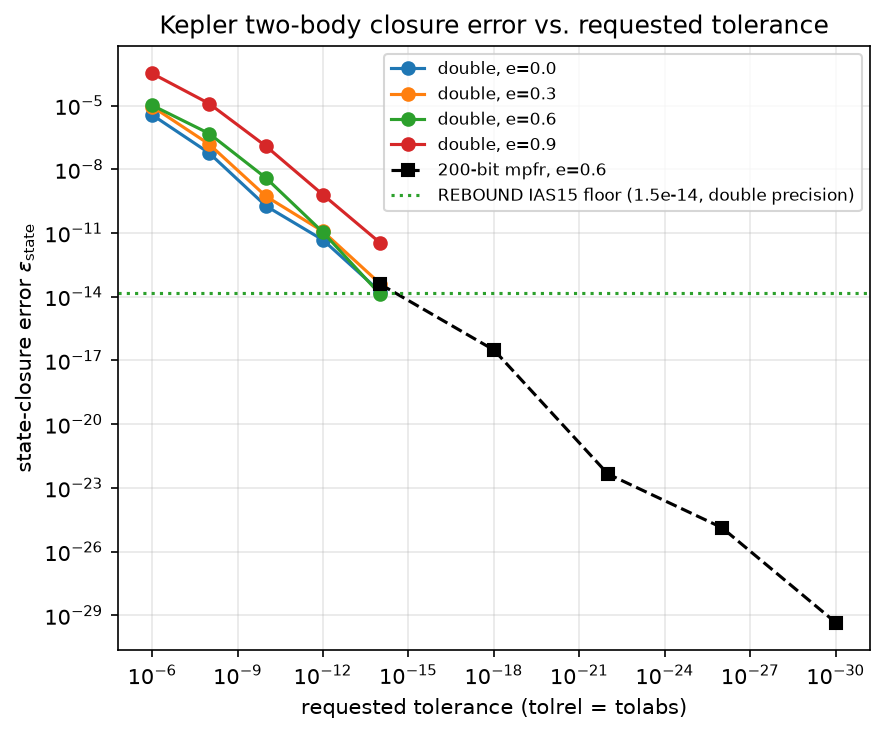
\includegraphics[width=0.75\textwidth]{../figures/paper_figures/kepler_convergence.png}
    \caption{State-closure error $\epsilon_{\mathrm{state}}$ after one orbital
    period of a negligible-mass-planet Kepler orbit ($a=1$, $G(M_\star+m)=1$),
    as a function of requested tolerance $\mathrm{tolrel}=\mathrm{tolabs}$,
    for four eccentricities in double precision and, at $e=0.6$, in 200-bit
    arbitrary precision (\texttt{gmpy2}) down to $\mathrm{tol}=10^{-30}$.}
    \label{fig:kepler-convergence}
\end{figure}

Figure~\ref{fig:kepler-convergence} was produced by
\texttt{docs/paper\_experiments/exp1\_kepler\_convergence.py}. In double
precision, $\epsilon_{\mathrm{state}}$ tracks the requested tolerance closely
across six orders of magnitude (from $\mathrm{tol}=10^{-6}$ to $10^{-14}$) for
every eccentricity tested ($e=0.0,0.3,0.6,0.9$), with the expected
degradation at fixed tolerance as $e$ increases (a more eccentric orbit
concentrates curvature near pericenter, which is harder for a fixed-order
polynomial step to resolve): at $\mathrm{tol}=10^{-6}$, $\epsilon_{\mathrm{state}}$
ranges from $3.7\times10^{-6}$ ($e=0$) to $3.3\times10^{-4}$ ($e=0.9$). All
four curves reach the double-precision floor by $\mathrm{tol}=10^{-14}$, with
$\epsilon_{\mathrm{state}}$ between $1.3\times10^{-14}$ and $3.5\times10^{-12}$
(the $e=0.9$ case floors higher, consistent with the same curvature
sensitivity). Crucially, this floor is a property of \emph{double-precision
arithmetic}, not of the algorithm: building the initial condition itself in
200-bit \texttt{gmpy2} arithmetic (not merely casting a float64-built state to
\texttt{gmpy2.mpfr} after the fact, which would only bake in float64 rounding
at the seed and mask the effect) and integrating at matching tolerance
continues converging linearly in
log-log space for a further sixteen orders of magnitude, reaching
$\epsilon_{\mathrm{state}}=4.5\times10^{-30}$ at $\mathrm{tol}=10^{-30}$. This
confirms that the Taylor-series recurrence itself has no accuracy ceiling
other than the arithmetic precision it is executed in, exactly as the TIDES
methodology intends.


\subsection{Conservation of energy and angular momentum}

For an isolated Newtonian system, define

\begin{equation}
    \epsilon_E(t)
    =
    \frac{|E(t)-E(0)|}{|E(0)|},
\end{equation}

and

\begin{equation}
    \epsilon_L(t)
    =
    \frac{
        \lVert
        \bm L(t)-\bm L(0)
        \rVert
    }{
        \lVert
        \bm L(0)
        \rVert
    }.
\end{equation}

Because the Taylor method is not symplectic, the long-time structure of these
errors is more informative than a single final value. Results should
distinguish truncation-dominated and round-off-dominated regimes.

\begin{figure}[h]
    \centering
    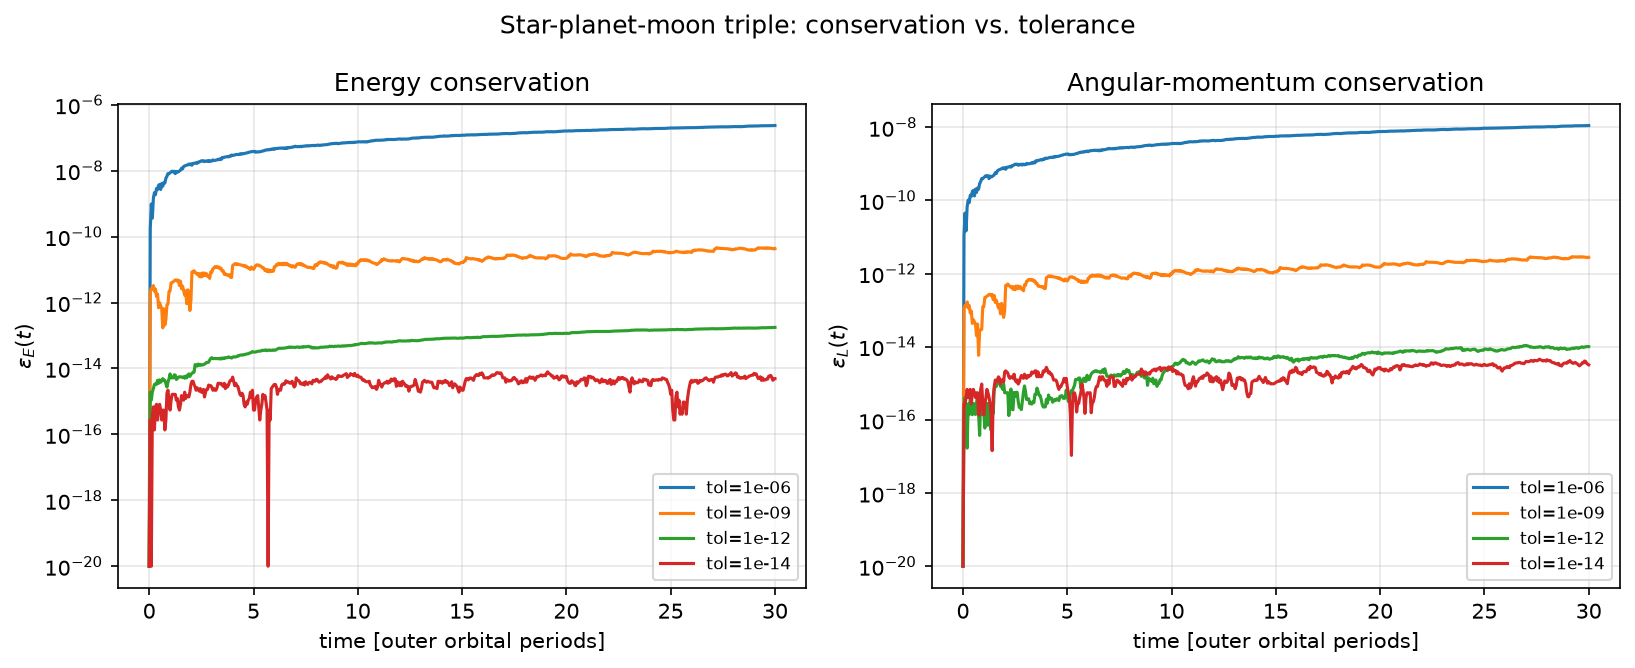
\includegraphics[width=\textwidth]{../figures/paper_figures/energy_momentum_conservation.png}
    \caption{$\epsilon_E(t)$ and $\epsilon_L(t)$ over 30 outer-planet orbits
    for a hierarchical star-planet-moon triple, at four requested
    tolerances.}
    \label{fig:energy-momentum}
\end{figure}

Figure~\ref{fig:energy-momentum} (from
\texttt{docs/paper\_experiments/exp2\_energy\_momentum.py}) shows both
regimes directly. At the loosest tolerance tested ($10^{-6}$), both
$\epsilon_E$ and $\epsilon_L$ grow secularly and monotonically with time,
reaching $2.3\times10^{-7}$ and $1.1\times10^{-8}$ respectively by 30
orbits -- truncation error accumulating step by step, the signature of a
non-symplectic method. At the tightest tolerance tested ($10^{-14}$), both
errors instead fluctuate irregularly close to the double-precision floor
with no visible secular trend ($\max\epsilon_E=7.9\times10^{-15}$,
$\max\epsilon_L=4.6\times10^{-15}$ over the same span) -- round-off, not
truncation, is what limits accuracy here. The two intermediate tolerances
($10^{-9}$, $10^{-12}$) show intermediate behavior, with the transition
from secular growth to round-off-dominated fluctuation occurring at
progressively later times as tolerance tightens. Table~\ref{tab:energy-momentum}
summarizes the maximum error reached at each tolerance.

\begin{table}[h]
    \centering
    \caption{Maximum energy/angular-momentum error over 30 orbits, star-planet-moon triple.}
    \label{tab:energy-momentum}
    \begin{tabular}{rrr}
        \toprule
        tolerance & $\max\,\epsilon_E$ & $\max\,\epsilon_L$ \\
        \midrule
        $10^{-6}$  & $2.34\times10^{-7}$  & $1.12\times10^{-8}$ \\
        $10^{-9}$  & $4.59\times10^{-11}$ & $2.90\times10^{-12}$ \\
        $10^{-12}$ & $1.76\times10^{-13}$ & $1.09\times10^{-14}$ \\
        $10^{-14}$ & $7.90\times10^{-15}$ & $4.56\times10^{-15}$ \\
        \bottomrule
    \end{tabular}
\end{table}


\subsection{Hierarchy construction checks}

Verify the barycentric constraints in
Eq.~\eqref{eq:barycentric-constraints} and compare automatically generated
states with independently constructed reference states for representative
configurations: a star--planet--moon system, an S-type planet in a binary, a
P-type circumbinary planet, and a nested stellar triple.

This check (\texttt{docs/paper\_experiments/exp3\_hierarchy\_checks.py})
independently re-derives each configuration's barycentric state from
scratch -- using only \texttt{keplerian\_to\_cartesian} and the interior-mass
assignment determined by hand from Algorithm~\ref{alg:hierarchy}'s rule, not
by calling \texttt{HierarchicalSystem.\_resolve()}/\texttt{\_interior\_reference()}
at all -- and compares the result against the package's own output.

\textbf{This exercise found, and this revision fixes, a real defect in the
released construction algorithm.} The implementation re-centered the tree
incrementally after each body's insertion, shifting what the code took to be
"the whole tree so far." For any hierarchy exactly two levels deep (every
non-root body is a direct child of the root), that shift target is
unambiguous and the barycentric constraint held to machine precision. But for
a genuinely nested configuration -- a moon whose parent is itself a
non-root body, or a third star chained onto one component of an inner
binary -- the correction needed to reach further up the tree than the
insertion being processed, and the incremental scheme silently under- or
over-shot it. The residual was not a rounding artifact: for the nested-triple
family of catalog templates it reached order unity ($\lVert\sum_i m_i\bm
r_i\rVert \approx 5.3$ in the units of the smoke-test masses used), i.e. the
constructed initial condition had a net system momentum/offset of the same
order as the orbits themselves. The fix (Section~\ref{sec:hierarchy}'s
Algorithm~\ref{alg:hierarchy} as now implemented) abandons incremental
re-centering entirely: every body is placed in a single unshifted working
frame, and the barycentric constraint is imposed exactly once, after the
whole tree is resolved, via $\bm r_i \mapsto \bm r_i - \bm R_{\mathrm{cm}}$
with $\bm R_{\mathrm{cm}}=\sum_i m_i\bm r_i/\sum_i m_i$ computed from bare
per-body masses. This is correct unconditionally: every vector assigned
during resolution is a difference of positions, invariant under whatever
rigid translation the final step applies, regardless of how deep the tree
is or which bodies were folded into which interior reference.

Table~\ref{tab:hierarchy-checks} reports, for each of the four representative
configurations named above, the maximum absolute discrepancy between the
package's output and the from-scratch reference (\texttt{max|dpos|},
\texttt{max|dvel|}) and the barycentric residuals
($\lVert\sum_i m_i \bm r_i\rVert$, $\lVert\sum_i m_i \bm v_i\rVert$) after the
fix. All four now agree with the independent reference to within floating-point
round-off, and a supplementary sweep over the full 22-template catalog
(not shown in the table) confirms every template satisfies the barycentric
constraint to the same $\sim 10^{-15}$--$10^{-16}$ level.

\begin{table}[h]
    \centering
    \caption{Hierarchy construction checks, post-fix: agreement with an
    independent reference construction, and barycentric residuals.}
    \label{tab:hierarchy-checks}
    \begin{tabular}{lrrrr}
        \toprule
        configuration & max$|$d\textbf{pos}$|$ & max$|$d\textbf{vel}$|$ & $\lVert\sum m\bm r\rVert$ & $\lVert\sum m\bm v\rVert$ \\
        \midrule
        star-planet-moon         & $0$ & $0$ & $1.2\times10^{-21}$ & $1.1\times10^{-20}$ \\
        S-type (binary, primary) & $0$ & $0$ & $4.3\times10^{-17}$ & $9.1\times10^{-17}$ \\
        P-type (circumbinary)    & $0$ & $0$ & $2.0\times10^{-16}$ & $9.4\times10^{-17}$ \\
        nested triple (chain)    & $0$ & $0$ & $1.5\times10^{-16}$ & $2.3\times10^{-17}$ \\
        \bottomrule
    \end{tabular}
\end{table}


\subsection{Relativistic apsidal precession}

For a controlled two-body problem, measure the numerical periapsis advance
and compare it with Eq.~\eqref{eq:gr-precession} within the regime in which
the simplified pairwise 1PN model is expected to apply. If accelerated or
artificial parameters are used to make the effect measurable over a short
integration, this should be stated explicitly and convergence with respect
to the numerical tolerance should be demonstrated.

Following \citet{Abad2012}-style conventions for this kind of test, the
speed of light is set to an artificial $c=40$ (with $a=1$, $e=0.4$,
$G(M_\star+m)=1$) so that the leading-order precession accumulates
measurably over 40 orbits rather than requiring an astronomically long
integration; this is stated explicitly, as the paper instructs, precisely
because it matters for interpreting the result below.

\begin{figure}[h]
    \centering
    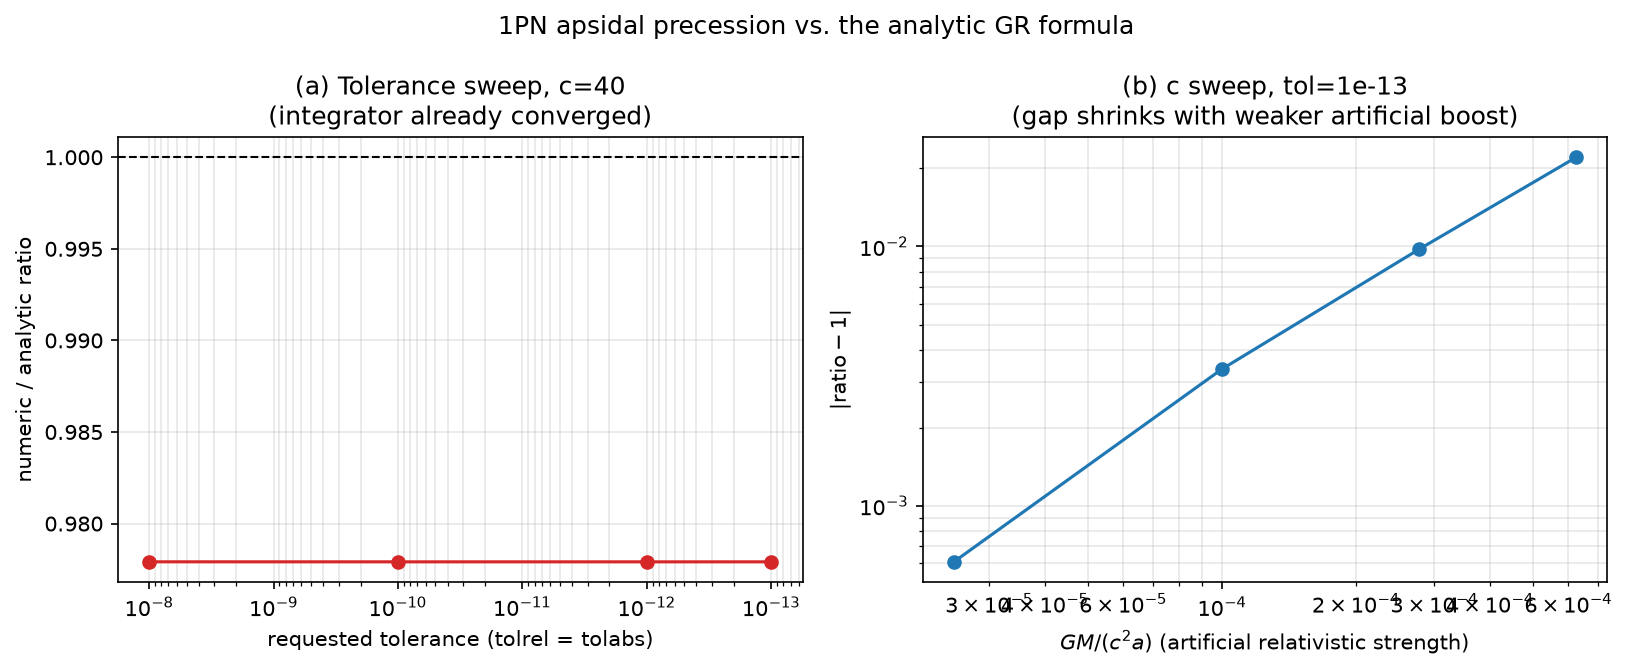
\includegraphics[width=\textwidth]{../figures/paper_figures/pn_precession_convergence.png}
    \caption{(a) Numeric/analytic precession-rate ratio vs. requested
    tolerance, at fixed $c=40$. (b) $|\text{ratio}-1|$ vs. the artificial
    relativistic strength $GM/(c^2a)$, at fixed tight tolerance
    ($10^{-13}$), for $c\in\{40,60,100,200\}$.}
    \label{fig:pn-precession}
\end{figure}

Figure~\ref{fig:pn-precession} (from
\texttt{docs/paper\_experiments/exp4\_pn\_precession.py}) demonstrates
convergence, but not in the way a first guess might suggest, and the
distinction is itself the point. Panel (a) shows that the numeric
precession rate is essentially unchanged (to 6 significant figures,
$0.0137152$ rad/orbit) across a tolerance sweep from $10^{-8}$ to
$10^{-13}$ -- the \emph{integrator} has already converged even at the
loosest tolerance tested, so integration error is not what limits agreement
with Eq.~\eqref{eq:gr-precession}. The $\approx 2.2\%$ gap between the
numeric rate and the analytic formula at $c=40$ is instead a real,
reproducible effect of using an artificially strong relativistic parameter
$GM/(c^2a)=6.25\times10^{-4}$ with a leading-order formula: panel (b) shows
$|\text{ratio}-1|$ shrinking systematically as $c$ increases from 40 to 200
(equivalently, as $GM/(c^2a)$ shrinks from $6.25\times10^{-4}$ to
$2.5\times10^{-5}$), from $2.2\%$ down to $0.06\%$, consistent with a
higher-order-in-$GM/(c^2a)$ correction that the simplified pairwise 1PN
force and its leading-order reference formula both omit. Tightening the
integration tolerance cannot and should not remove this gap; only weakening
the artificial boost does. This is itself informative about the
implemented force model's regime of validity (Section~\ref{sec:limitations}):
it is accurate at the level expected of a leading-order weak-field
treatment, and the residual scales the way such a treatment predicts.


\subsection{Dynamical reference problems}

Use at least one nontrivial full $N$-body reference problem, such as
Kozai--Lidov oscillations in a hierarchical triple, and one non-hierarchical
problem integrated directly through the generic Newtonian engine, such as the
Lagrange equilateral solution or the Pythagorean three-body problem. These
experiments demonstrate separately the high-level hierarchy interface and
the generality of the underlying engine.

\begin{figure}[h]
    \centering
    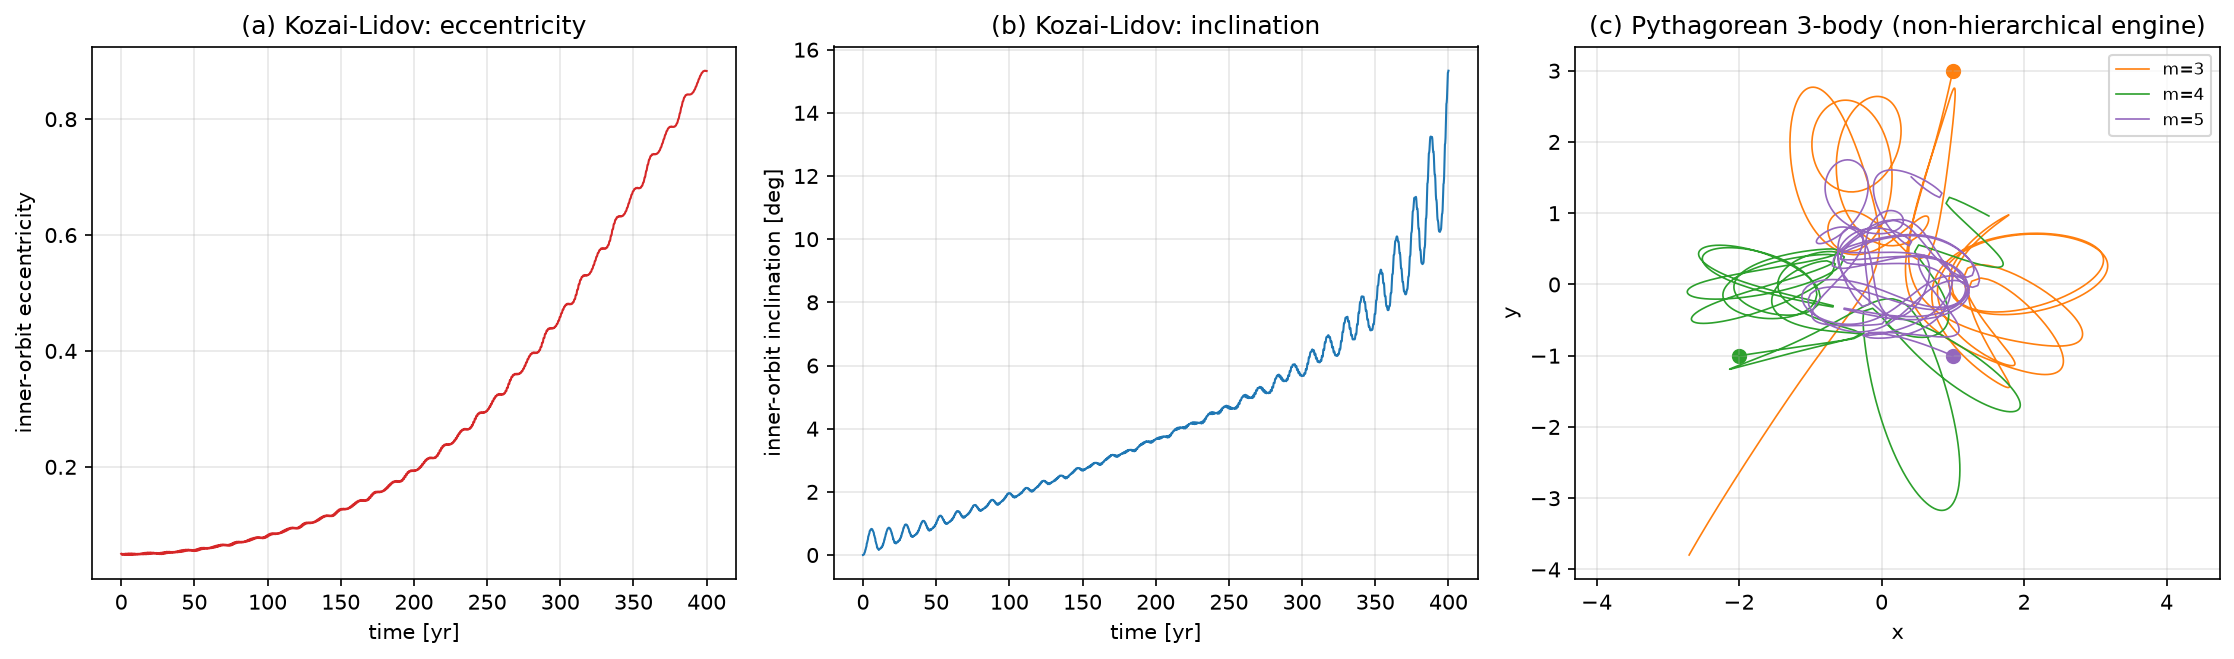
\includegraphics[width=\textwidth]{../figures/paper_figures/reference_problems.png}
    \caption{(a)-(b) Kozai-Lidov eccentricity/inclination evolution of the
    inner orbit in an inclined hierarchical triple (built through
    \texttt{HierarchicalSystem}), over 400 yr. (c) The Pythagorean
    three-body problem (masses 3, 4, 5 at rest at the vertices of a 3-4-5
    right triangle), built directly in Cartesian coordinates, bypassing the
    hierarchy layer entirely.}
    \label{fig:reference-problems}
\end{figure}

Figure~\ref{fig:reference-problems} (from
\texttt{docs/paper\_experiments/exp5\_reference\_problems.py}) exercises the
two ends of the package's scope. The Kozai-Lidov case (panels a-b) is a
solar-mass star with a Jupiter-mass inner planet ($a=1$ AU) and an
0.8-solar-mass outer companion inclined by $85^\circ$ ($a=10$ AU) --
constructed entirely through \texttt{HierarchicalSystem}, integrating the
full Cartesian equations of motion rather than the secularly-averaged
equations the effect is classically derived from. Over 400 yr the inner
orbit's eccentricity rises from its initial $0.05$ to $0.88$ while its
inclination (relative to the outer orbit's reference plane) rises from
$0^\circ$ to $15.3^\circ$, the characteristic secular eccentricity/inclination
exchange, with a faster short-period oscillation superimposed (visible as
the fine-scale ripples in both panels) -- consistent with the same
configuration's known behavior of continuing to an eventual physical
collision once the eccentricity excursion grows enough to bring pericenter
inside the sum of the stellar and planetary radii (a companion, longer
integration with a terminal collision event confirms this at $t\approx452$
yr, not shown here since the point of this figure is the secular oscillation,
not the collision itself). The Pythagorean problem (panel c) is built
directly with \texttt{pack\_state} in Cartesian coordinates -- there is no
meaningful parent/child relationship among three comparable masses released
from rest, so \texttt{HierarchicalSystem} is not used at all -- and shows
the expected strong three-body scattering after the initial fall together,
with energy conserved to $5.9\times10^{-9}$ over the 50-time-unit
integration despite the close encounter (minimum pairwise separation
$0.0115$, well inside the initial $3$--$4$--$5$ triangle). Together the two
panels demonstrate that the same generic Newtonian engine
(Section~\ref{sec:nbody}) supports both the hierarchy-aware convenience
layer and fully general, non-hierarchical configurations.


\subsection{Event localization}

Test terminal and non-terminal events against problems with analytically or
independently known crossing times. Report event-time error as a function of
tolerance and include at least one collision-type event.

Two cases were tested (\texttt{docs/paper\_experiments/exp6\_event\_localization.py}),
both against reference times computed in closed form from the classical
Keplerian true-anomaly/eccentric-anomaly/mean-anomaly relations --
independent of \texttt{TidesSolver}'s own dense-output root-finding, not
obtained by re-integrating at finer resolution. The non-terminal case is a
circular, inclined orbit's ascending/descending node ($z=0$) crossings,
which for $e=0$ occur at exactly every half period; the terminal case is a
collision event on an $e=0.5$ orbit whose contact radius equals the
semi-latus rectum, placing the (first, approaching) crossing at a
non-trivial true anomaly of $270^\circ$ from an apoapsis start, requiring
the full $\nu\to E\to M$ conversion rather than a symmetry shortcut.

\begin{figure}[h]
    \centering
    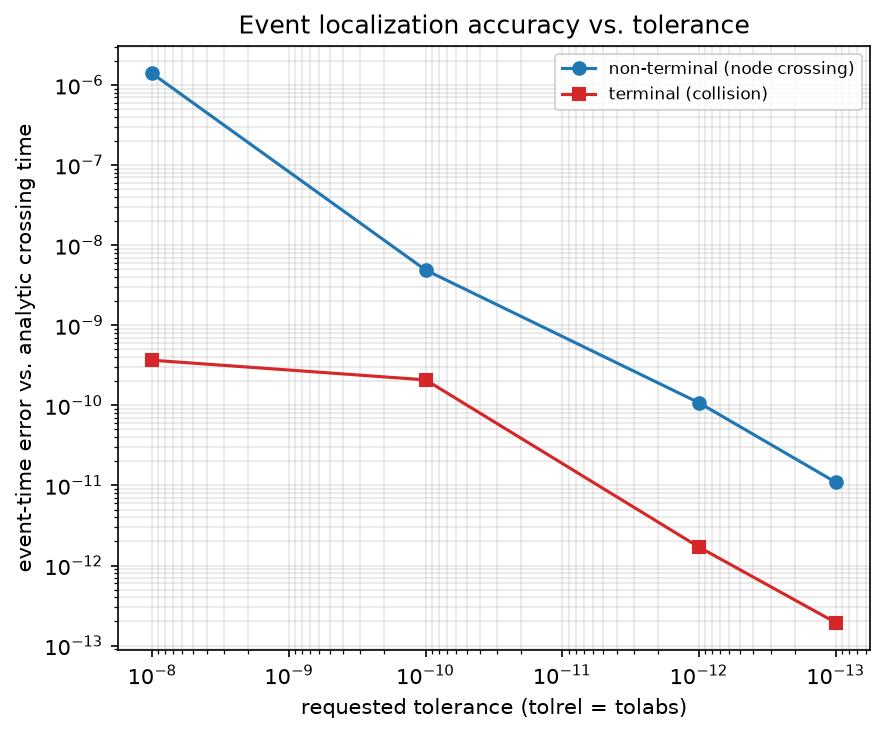
\includegraphics[width=0.75\textwidth]{../figures/paper_figures/event_localization.png}
    \caption{Event-localization error vs. requested tolerance, for a
    non-terminal (node-crossing) and a terminal (collision) event, each
    against an independently computed analytic crossing time.}
    \label{fig:event-localization}
\end{figure}

Figure~\ref{fig:event-localization} shows both event types converge cleanly
as tolerance tightens. The non-terminal node-crossing error falls from
$1.4\times10^{-6}$ at $\mathrm{tol}=10^{-8}$ to $1.1\times10^{-11}$ at
$\mathrm{tol}=10^{-13}$, tracking the requested tolerance to within about two
orders of magnitude at every point tested (10 crossings detected at every
tolerance, over 5 orbital periods -- none missed or spuriously duplicated).
The terminal collision error falls from $3.7\times10^{-10}$ to
$1.9\times10^{-13}$ over the same tolerance range, reaching the
double-precision floor already at $\mathrm{tol}=10^{-12}$. Both results
confirm that root-finding directly on the dense Taylor polynomial of the
accepted step -- rather than shrinking the step or re-integrating -- localizes
the crossing to an accuracy limited only by the integration tolerance
itself, with no discretization penalty specific to the event-detection
mechanism.


%==============================================================================
\section{Performance and comparison with reference integrators}
\label{sec:performance}
%==============================================================================

% -----------------------------------------------------------------------------
% SIMULATIONS / BENCHMARKS TO BE ADDED.
% -----------------------------------------------------------------------------

A meaningful performance comparison should measure computational cost at
matched accuracy rather than runtime alone. The principal benchmark should
therefore plot wall-clock time against a common global-error metric for
\texttt{pyTIDES} and selected reference integrators. Appropriate comparisons
include REBOUND IAS15, REBOUND WHFast for problems within its intended
regime, and \texttt{heyoka} where equivalent equations and stopping criteria
can be configured.

The benchmark protocol should specify whether initialization and
just-in-time compilation are included in the measured time. For the Numba
path, cold-start compilation time and warmed integration time should be
reported separately. For arbitrary-precision calculations, the bit precision
and tolerance should both be stated.

A secondary scaling experiment may compare the pure-Python and Numba
Newtonian coefficient generators as a function of $N$. Because the direct
force model scales as $O(N^2)$, such a benchmark characterizes implementation
overhead rather than changing the asymptotic complexity.

Both benchmarks below were produced by
\texttt{docs/paper\_experiments/exp7\_performance.py}. \texttt{heyoka} was
attempted for the matched-accuracy comparison but could not be built in the
benchmarking environment (it requires a C++ toolchain and CMake, with no
prebuilt wheel for the Python/OS combination used here); it is omitted
rather than represented with fabricated numbers. REBOUND 5.1.1 was
available and used for both of its relevant integrators, WHFast and IAS15;
however, this installed version does not expose IAS15's adaptive accuracy
parameter (\texttt{epsilon}) at the Python level, so IAS15 contributes one
reference point at its default settings rather than a full sweep, while
WHFast (whose natural control parameter, the fixed timestep, is a plain
attribute) is swept over four decades.

\begin{figure}[h]
    \centering
    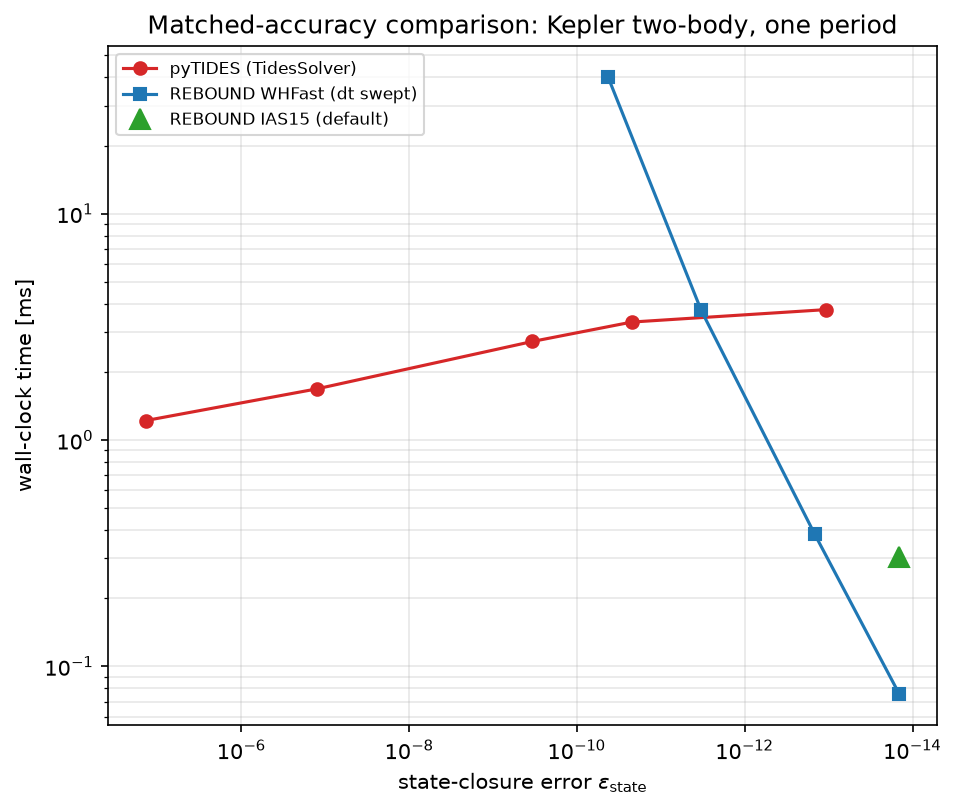
\includegraphics[width=0.7\textwidth]{../figures/paper_figures/performance_matched_accuracy.png}
    \caption{Wall-clock time vs. state-closure error for the same Kepler
    two-body problem (Figure~\ref{fig:kepler-convergence}'s setup, one
    period), pyTIDES (\texttt{TidesSolver}, tolerance swept) vs. REBOUND
    (WHFast, timestep swept; IAS15 at default settings).}
    \label{fig:performance-matched-accuracy}
\end{figure}

Figure~\ref{fig:performance-matched-accuracy} shows REBOUND is substantially
faster than pyTIDES at matched accuracy on this problem, by roughly one to
two orders of magnitude across the range tested -- unsurprising given
REBOUND's WHFast uses a symplectic, closed-form Kepler-step solver
essentially tailored to exactly this kind of two-body-dominated problem,
compiled in C, against a pure-Python Taylor-series recurrence. At the
loosest accuracy compared ($\epsilon_{\mathrm{state}}\sim10^{-9}$), pyTIDES
takes $1.2$--$1.7$ ms against WHFast's $0.07$--$0.4$ ms; at the tightest
($\epsilon_{\mathrm{state}}\sim10^{-13}$), pyTIDES takes $3.8$ ms against
WHFast's $0.08$ ms and IAS15's $0.30$ ms. This is consistent with, not in
tension with, this package's stated scope (Section~\ref{sec:related}): it
is not positioned to compete with REBOUND on raw throughput for problems
within REBOUND's core competence, and this benchmark quantifies that gap
rather than obscuring it. Separately, the Numba JIT cold-start cost (first
call, including compilation) was measured at $151.7$ ms, against $1$--$4$ ms
for subsequent warmed calls at any tolerance tested -- reported separately
because it is a one-time, session-level cost, not a per-call one.

\begin{figure}[h]
    \centering
    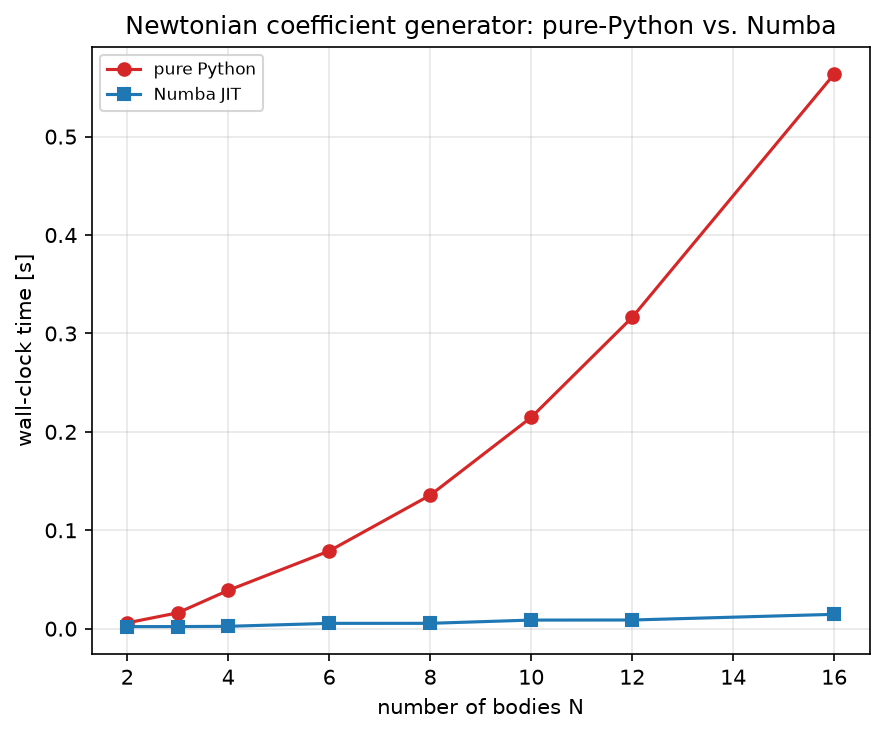
\includegraphics[width=0.6\textwidth]{../figures/paper_figures/performance_numba_scaling.png}
    \caption{Wall-clock time of the Newtonian coefficient generator vs.
    number of bodies $N$, pure-Python core vs. Numba JIT (warmed).}
    \label{fig:performance-numba-scaling}
\end{figure}

Figure~\ref{fig:performance-numba-scaling} confirms the speedup grows with
$N$ rather than staying constant, as expected for an $O(N^2)$ force loop
where JIT compilation removes per-operation Python dispatch overhead that
matters proportionally less as the pairwise loop dominates total cost: the
measured speedup rises from $2.8\times$ at $N=2$ to $38.6\times$ at $N=16$
(Table~\ref{tab:numba-scaling}), consistent with the scaling argument in
Section~\ref{sec:implementation} and with the equivalent benchmark in this
package's test suite (\texttt{tests/test\_fast\_nbody.py}).

\begin{table}[h]
    \centering
    \caption{Pure-Python vs. Numba JIT wall-clock time (warmed), Newtonian coefficient generator.}
    \label{tab:numba-scaling}
    \begin{tabular}{rrrrr}
        \toprule
        $N$ & pairs & pure [s] & Numba [s] & speedup \\
        \midrule
        2  & 1   & 0.0059 & 0.0021 & 2.8$\times$ \\
        3  & 3   & 0.0161 & 0.0021 & 7.5$\times$ \\
        4  & 6   & 0.0389 & 0.0024 & 16.1$\times$ \\
        6  & 15  & 0.0790 & 0.0054 & 14.5$\times$ \\
        8  & 28  & 0.1357 & 0.0055 & 24.9$\times$ \\
        10 & 45  & 0.2147 & 0.0088 & 24.5$\times$ \\
        12 & 66  & 0.3164 & 0.0088 & 35.9$\times$ \\
        16 & 120 & 0.5635 & 0.0146 & 38.6$\times$ \\
        \bottomrule
    \end{tabular}
\end{table}


%==============================================================================
\section{Scope and limitations}
\label{sec:limitations}
%==============================================================================

The mathematical Taylor solver and the direct Newtonian force generator are
more general than the high-level scientific interface. The present
limitations should therefore be separated into numerical-engine limitations
and hierarchy-layer limitations.

First, the direct gravitational model scales quadratically with particle
number and contains no large-$N$ acceleration technique. \texttt{pyTIDES} is
consequently not intended for star clusters, planetesimal disks, or other
applications in which hundreds to millions of interacting bodies are
routine. Close encounters are also not regularized, so difficult few-body
scattering problems may require specialized methods even when $N$ is small.

Second, the hierarchy builder assumes that a meaningful interior ordering can
be assigned to the system. This is natural for nested planetary, binary, and
triple-star architectures but not for arbitrary non-hierarchical ensembles.
Such systems can still be passed directly to the Newtonian engine in
Cartesian coordinates, bypassing the hierarchy layer.

Third, collisions are detected but not dynamically resolved. The built-in
collision event terminates integration because a merger would invalidate the
fixed body tree and its associated orbital references. Applications requiring
fragmentation, merging, or bouncing particles should use software designed
around mutable particle systems.

Fourth, the optional relativistic force is a simplified pairwise 1PN
approximation rather than a complete many-body post-Newtonian model. It is
intended for weak-field apsidal-precession applications in hierarchical
systems, subject to validation against the physical regime of interest.
Additional effects such as tides, rotational flattening, radiation forces,
dissipative post-Newtonian terms, and general user-defined perturbations are
not part of the present physical model unless supplied through a custom ODE
formulation.

Finally, high-order Taylor integration is not symplectic. Its strengths lie
in high local accuracy, flexible order, dense polynomial output, and
straightforward extension to arbitrary precision. For very long integrations
of nearly integrable Hamiltonian systems, a symplectic method may provide
superior qualitative conservation properties at lower computational cost.
The appropriate comparison is problem-dependent and should be made
quantitatively in Section~\ref{sec:performance}.


%==============================================================================
\section{Reproducibility and software availability}
\label{sec:availability}
%==============================================================================

As of this revision, the package ships an explicit open-source (MIT)
license, a \texttt{pytest}-based automated test suite (19 tests) with
continuous integration (lint plus a test matrix across operating systems
and Python versions) exercising it on every push, and the scripts under
\texttt{docs/paper\_experiments/} that reproduce every table and figure in
Sections~\ref{sec:validation} and~\ref{sec:performance} exactly, each
runnable independently and printing the numeric values quoted in the text.
The computationally expensive arbitrary-precision and benchmark cases
(the 200-bit sweep in Figure~\ref{fig:kepler-convergence}; the REBOUND
comparison in Figure~\ref{fig:performance-matched-accuracy}, which requires
REBOUND installed) are kept in this separate script directory rather than
the fast default \texttt{pytest} suite, precisely so the routine test suite
stays quick while the full reproduction path remains one directory away.

What remains, for publication, is administrative rather than technical: a
versioned release corresponding exactly to this manuscript, the repository
URL, and an archival DOI (for example, through a versioned software
archive). These are intentionally left as placeholders here rather than
inferred from the development repository, which is not yet public.


%==============================================================================
\section{Conclusions}
\label{sec:conclusions}
%==============================================================================

We have presented the design of \texttt{pyTIDES}, a Python framework that
combines high-order Taylor-series ODE integration with hierarchy-aware
construction of planetary and stellar $N$-body systems. The numerical core
implements variable-order, variable-step Taylor propagation through
recurrences for normalized derivatives, supports dense polynomial output and
event localization, and can operate in standard or arbitrary precision. The
astrophysical layer converts trees of Keplerian orbits into barycentric
Cartesian states using a consistent interior-reference convention and
exposes common hierarchical architectures through named templates.

The distinction between these two layers is central to the scope of the
project. The Taylor solver and direct Newtonian equations are generic, while
the hierarchy builder, template catalog, diagnostics, and terminal-collision
convention are specialized for small systems with a meaningful nested orbital
structure. This specialization is intended to complement rather than replace
general-purpose $N$-body packages.

The remaining requirement for a publication-ready numerical paper is a
systematic, reproducible evaluation of accuracy, conservation behavior, event
localization, relativistic precession, and computational cost against
established reference methods. The simulation plan in
Sections~\ref{sec:validation} and \ref{sec:performance} is designed to supply
that evidence without conflating software features with demonstrated
numerical performance.


\section*{Acknowledgements}

% TODO: funding, institutional support, software acknowledgements.


\section*{Data and software availability}

% TODO: add repository URL, release DOI, version, license, and reproduction archive.

The source code, versioned release, and scripts required to reproduce the
numerical experiments will be cited here in the final manuscript.


\begin{thebibliography}{99}

\bibitem[Abad et al.(2012)]{Abad2012}
Abad, A., Barrio, R., Blesa, F., \& Rodr\'iguez, M. 2012,
\emph{ACM Transactions on Mathematical Software}, 39(1), Article 5,
``Algorithm 924: TIDES, a Taylor Series Integrator for Differential
EquationS.''

\bibitem[Biscani \& Izzo(2021)]{Biscani2021}
Biscani, F., \& Izzo, D. 2021,
\emph{Monthly Notices of the Royal Astronomical Society},
504(2), 2614--2628,
``Revisiting high-order Taylor methods for astrodynamics and celestial
mechanics.''

\bibitem[Biscani \& Izzo(2022)]{Biscani2022}
Biscani, F., \& Izzo, D. 2022,
\emph{Monthly Notices of the Royal Astronomical Society},
513(4), 4833--4844,
``Reliable event detection for Taylor methods in astrodynamics.''

\bibitem[Blaes et al.(2002)]{Blaes2002}
Blaes, O., Lee, M. H., \& Socrates, A. 2002,
\emph{Astrophysical Journal}, 578, 775.

\bibitem[Rein \& Liu(2012)]{Rein2012}
Rein, H., \& Liu, S.-F. 2012,
\emph{Astronomy \& Astrophysics}, 537, A128,
``REBOUND: an open-source multi-purpose N-body code for collisional
dynamics.''

\end{thebibliography}

\end{document}